\documentclass[tikz,border=8pt]{standalone}
% Shared look for every TikZ diagram. Load with % Shared look for every TikZ diagram. Load with % Shared look for every TikZ diagram. Load with \input{../../tools/tikz-style.tex}
\usepackage[T1]{fontenc}
\usepackage{lmodern}
\renewcommand{\sfdefault}{lmr}  % diagrams use the same serif as the text
\usetikzlibrary{arrows.meta, positioning, shapes.geometric, calc, fit, backgrounds}
\definecolor{cblue}{HTML}{4C78A8}
\definecolor{corange}{HTML}{F58518}
\definecolor{cgreen}{HTML}{54A24B}
\definecolor{cred}{HTML}{E45756}
\definecolor{cpurple}{HTML}{B279A2}
\definecolor{cgrey}{HTML}{6B6B6B}
\tikzset{
  every picture/.style={font=\sffamily, line width=1.2pt},
  box/.style={draw=#1, fill=#1!12, rounded corners=4pt, align=center, inner sep=7pt, minimum height=1.1cm},
  box/.default=cgrey,
  arrow/.style={-{Stealth[length=3mm]}, draw=cgrey, line width=1.4pt},
  title/.style={font=\sffamily\bfseries\Large},
  note/.style={font=\sffamily\small, text=cgrey, align=center},
}
\AtBeginDocument{\hyphenpenalty=10000 \exhyphenpenalty=10000}

\usepackage[T1]{fontenc}
\usepackage{lmodern}
\renewcommand{\sfdefault}{lmr}  % diagrams use the same serif as the text
\usetikzlibrary{arrows.meta, positioning, shapes.geometric, calc, fit, backgrounds}
\definecolor{cblue}{HTML}{4C78A8}
\definecolor{corange}{HTML}{F58518}
\definecolor{cgreen}{HTML}{54A24B}
\definecolor{cred}{HTML}{E45756}
\definecolor{cpurple}{HTML}{B279A2}
\definecolor{cgrey}{HTML}{6B6B6B}
\tikzset{
  every picture/.style={font=\sffamily, line width=1.2pt},
  box/.style={draw=#1, fill=#1!12, rounded corners=4pt, align=center, inner sep=7pt, minimum height=1.1cm},
  box/.default=cgrey,
  arrow/.style={-{Stealth[length=3mm]}, draw=cgrey, line width=1.4pt},
  title/.style={font=\sffamily\bfseries\Large},
  note/.style={font=\sffamily\small, text=cgrey, align=center},
}
\AtBeginDocument{\hyphenpenalty=10000 \exhyphenpenalty=10000}

\usepackage[T1]{fontenc}
\usepackage{lmodern}
\renewcommand{\sfdefault}{lmr}  % diagrams use the same serif as the text
\usetikzlibrary{arrows.meta, positioning, shapes.geometric, calc, fit, backgrounds}
\definecolor{cblue}{HTML}{4C78A8}
\definecolor{corange}{HTML}{F58518}
\definecolor{cgreen}{HTML}{54A24B}
\definecolor{cred}{HTML}{E45756}
\definecolor{cpurple}{HTML}{B279A2}
\definecolor{cgrey}{HTML}{6B6B6B}
\tikzset{
  every picture/.style={font=\sffamily, line width=1.2pt},
  box/.style={draw=#1, fill=#1!12, rounded corners=4pt, align=center, inner sep=7pt, minimum height=1.1cm},
  box/.default=cgrey,
  arrow/.style={-{Stealth[length=3mm]}, draw=cgrey, line width=1.4pt},
  title/.style={font=\sffamily\bfseries\Large},
  note/.style={font=\sffamily\small, text=cgrey, align=center},
}
\AtBeginDocument{\hyphenpenalty=10000 \exhyphenpenalty=10000}

% The Algorithm chooser view of the Course map. Hand-drawn: a decision flowchart cannot be generated sensibly.
% DRAFT: each recommendation is checked against its Note when that Note is written.
\begin{document}
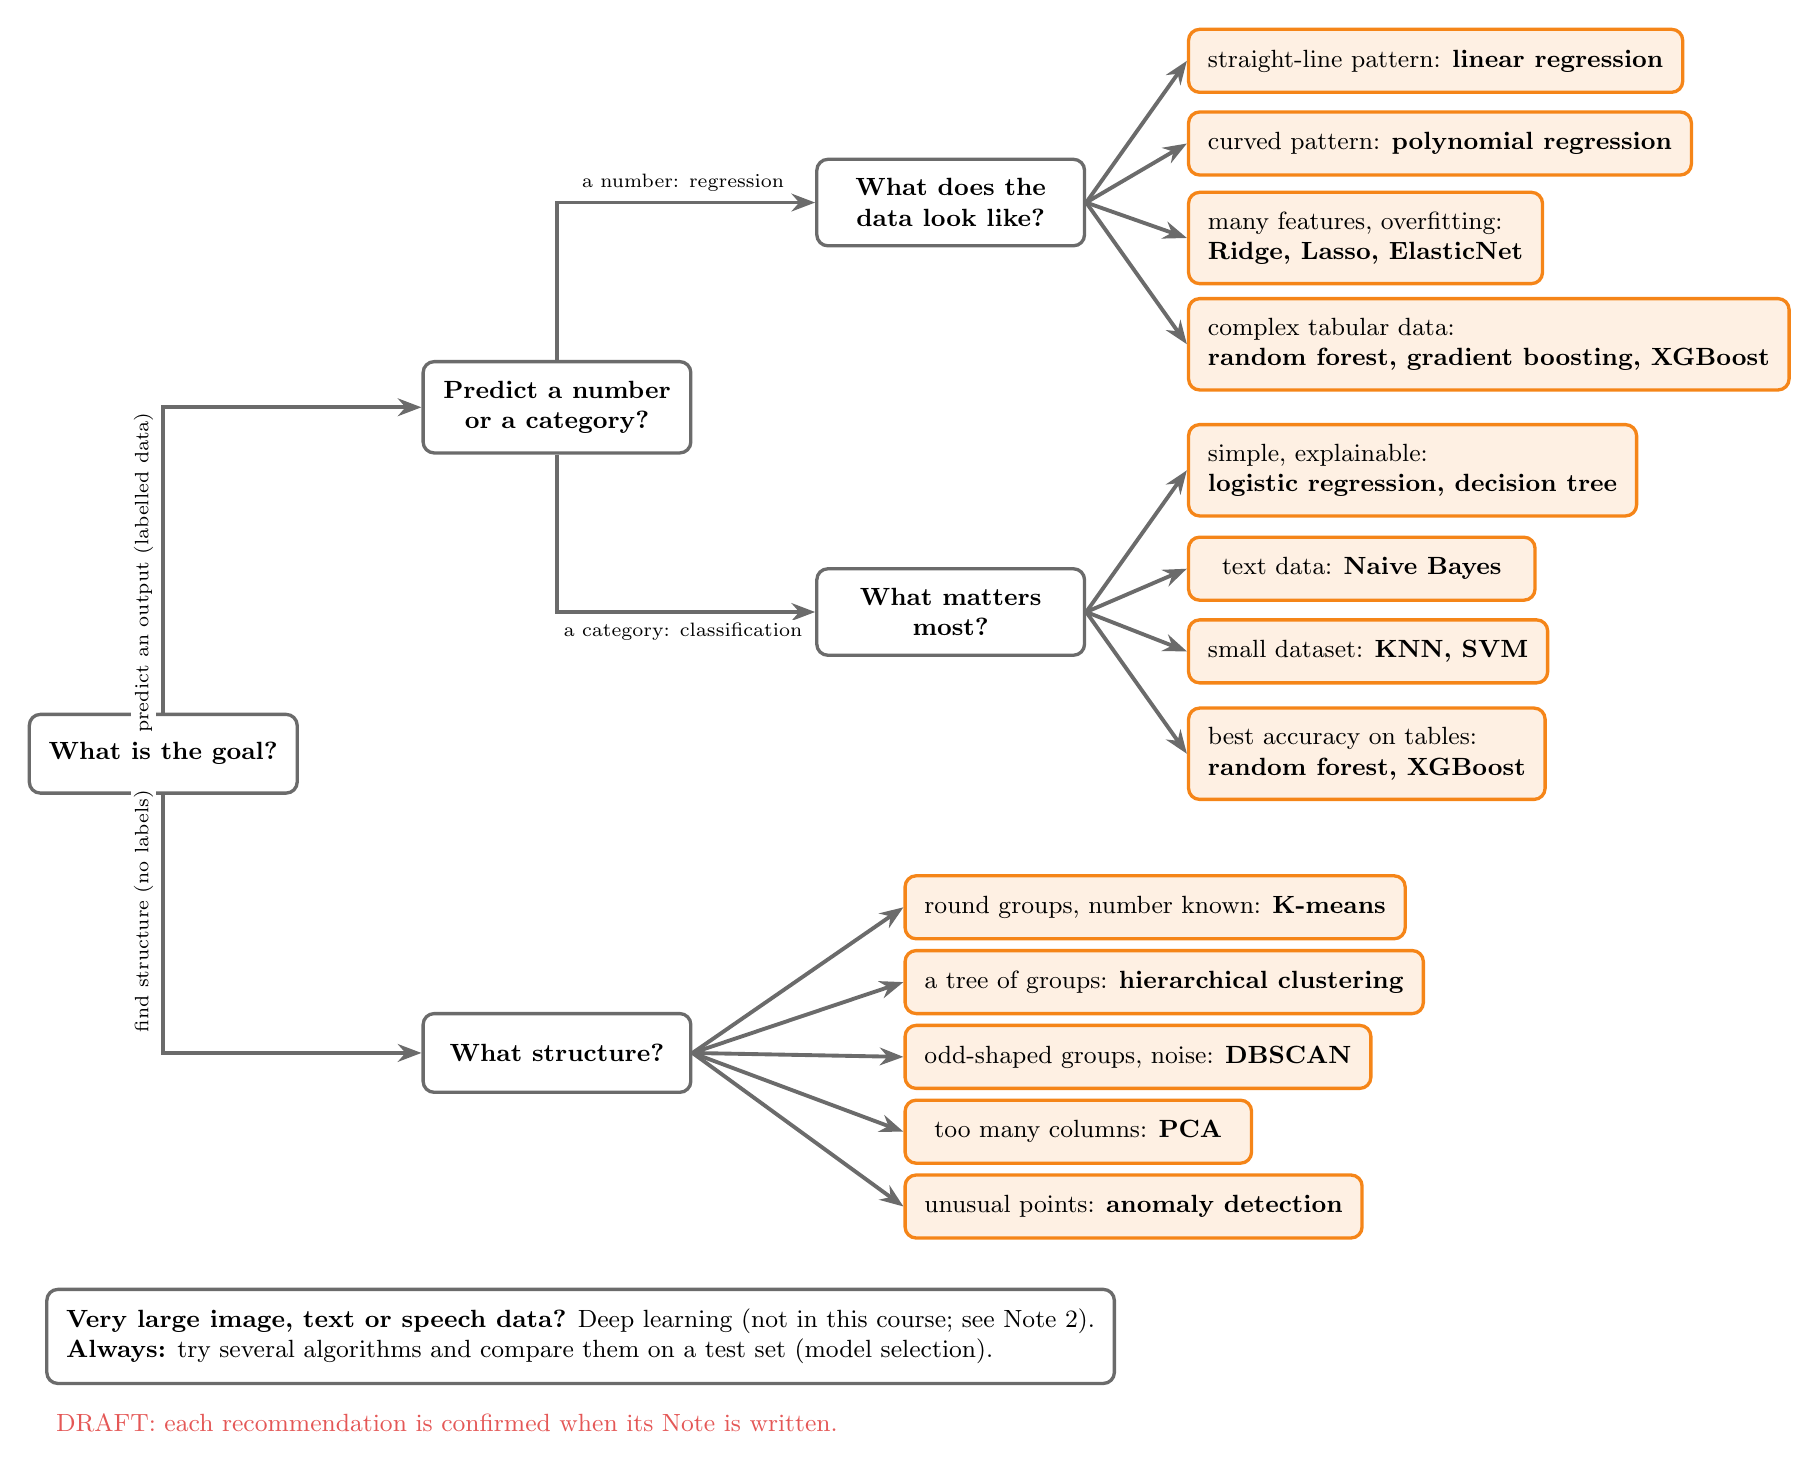
\begin{tikzpicture}[
    q/.style={box=cgrey, fill=white, minimum width=3.4cm, minimum height=1.0cm, font=\small\bfseries},
    alg/.style={box=corange, minimum width=4.4cm, minimum height=0.8cm, font=\small, align=left, anchor=west},
    lab/.style={note, text=black, font=\scriptsize, fill=white, inner sep=1pt}]
  \node[q, minimum width=3.0cm] (start) at (0,0) {What is the goal?};

  % ---- labelled data: predict an output
  \node[q] (task) at (5.0,4.4) {Predict a number\\or a category?};
  \draw[arrow] (start.north) |- (task.west);
  \node[lab, rotate=90] at (-0.25,2.3) {predict an output (labelled data)};

  \node[q] (num) at (10.0,7.0) {What does the\\data look like?};
  \draw[arrow] (task.north) |- (num.west);
  \node[lab] at (6.6,7.25) {a number: regression};
  \foreach \y/\t in {8.8/{straight-line pattern: \textbf{linear regression}},
                     7.75/{curved pattern: \textbf{polynomial regression}},
                     6.55/{many features, overfitting:\\\textbf{Ridge, Lasso, ElasticNet}},
                     5.2/{complex tabular data:\\\textbf{random forest, gradient boosting, XGBoost}}}
    { \node[alg] at (13.0,\y) {\t}; \draw[arrow] (num.east) -- (13.0,\y); }

  \node[q] (cat) at (10.0,1.8) {What matters\\most?};
  \draw[arrow] (task.south) |- (cat.west);
  \node[lab] at (6.6,1.55) {a category: classification};
  \foreach \y/\t in {3.6/{simple, explainable:\\\textbf{logistic regression, decision tree}},
                     2.35/{text data: \textbf{Naive Bayes}},
                     1.3/{small dataset: \textbf{KNN, SVM}},
                     0.0/{best accuracy on tables:\\\textbf{random forest, XGBoost}}}
    { \node[alg] at (13.0,\y) {\t}; \draw[arrow] (cat.east) -- (13.0,\y); }

  % ---- no labels: find structure
  \node[q] (unl) at (5.0,-3.8) {What structure?};
  \draw[arrow] (start.south) |- (unl.west);
  \node[lab, rotate=90] at (-0.25,-2.0) {find structure (no labels)};
  \foreach \y/\t in {-1.95/{round groups, number known: \textbf{K-means}},
                     -2.9/{a tree of groups: \textbf{hierarchical clustering}},
                     -3.85/{odd-shaped groups, noise: \textbf{DBSCAN}},
                     -4.8/{too many columns: \textbf{PCA}},
                     -5.75/{unusual points: \textbf{anomaly detection}}}
    { \node[alg] at (9.4,\y) {\t}; \draw[arrow] (unl.east) -- (9.4,\y); }

  \node[box=cgrey, fill=white, font=\small, align=left, anchor=west] at (-1.5,-7.4)
    {\textbf{Very large image, text or speech data?} Deep learning (not in this course; see Note 2).\\
     \textbf{Always:} try several algorithms and compare them on a test set (model selection).};
  \node[note, text=cred, anchor=west] at (-1.5,-8.5) {DRAFT: each recommendation is confirmed when its Note is written.};
\end{tikzpicture}
\end{document}
